% Chapter 2

\chapter{MiRNAs target prediction computational methods} % Main chapter title

\label{Chapter2} % For referencing the chapter elsewhere, use \ref{Chapter2} 


%----------------------------------------------------------------------------------------

\section{Introduction}
Earlier in Chapter~\ref{Chapter1} we described how miRNAs play a fundamental role in gene regulation. It is common belief that the final and probably most relevant step in their regulatory pathway is targeting \cite{computational_methods}. Targeting is intended as the binding of the mature miRNA to the messenger RNA via the RNA Induced Silencing Complex (see figure \ref{fig:mirna_binding}). Hence, valid targets need to be identified for miRNAs in order to properly understand their role in cellular pathways. 

However, many of the discovered miRNAs do not yet have identified targets. This is especially the case in animals where the miRNA does not bind to its target with a nearly perfect matching as it does in plants \cite{perfect_matching}. Experiments have proved that a single miRNA has the potential to regulate hundreds of target mRNAs and multiple miRNAs may compete for the regulation of the same mRNA \cite{multiple_binds}, however target validation is difficult, expensive, and time consuming. Thus, having considered all these facts, it is of crucial importance to have accurate computational miRNA target predictions.

\begin{figure}[hbt!]
	\centering
	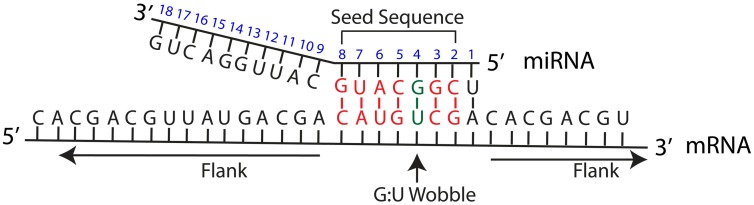
\includegraphics[width=0.7\textwidth]{Figures/seed_match}
	\caption{Example of miRNA targeting.}
	\label{fig:mirna_binding}
\end{figure}

%----------------------------------------------------------------------------------------

\section{MiRNA target prediction}
Before miRNA target prediction tools were available, possible miRNA binding sites were
determined manually. These target sites were later confirmed by laborious and inefficient techniques such as site-directed mutagenesis and other experimental methods. The identification of the first targets for the let-7 and lin-4 miRNAs led to the idea that miRNAs have a pattern in targeting genes which could be used to develop target prediction algorithms \cite{first_predictions}.

Originally gene targeting by miRNAs was believed to be the result of their binding to the 3'UTR of the target mRNA \cite{multiple_binds}, however recent studies \cite{grosswendt} have confirmed gene regulation as a result of the binding of the miRNA to the coding region as well as to the 5'UTR. Furthermore, computational evidence suggests that regulation via the binding of the miRNA to the coding region differs in comparison to the binding pattern seen at the 3'UTR. In particular, it's suggested that miRNAs target the coding regions of mRNAs with short 3'UTRs \cite{functional_sites}.

Another key factor in target prediction is that 3'UTRs are prone to change under different conditions which might result in the elimination of the target site. Binding in the coding region on the other hand may instead present an evolutionary advantage for the cell as it could help in the preservation of the miRNA binding site \cite{mirna_targets}.

\subsection{The importance of the seed region}
Targeting patterns are very different between plants and animals. Plants, in fact, show a near perfect complement between their miRNA and the respective target mRNA. On the other hand animal miRNAs bind their targets with only partial complementarity. In particular, a region of about 6 to 8 nucleotides in length at the beginning of the miRNA is of crucial importance in the targeting.  This short subsequence is called \emph{seed region} and it comprises the nucleotides between the second at the eighth (the seed sequence in Figure \ref{fig:mirna_binding}). 

The seed region is very important because it binds to the target mRNA leading to the regulation of the gene in question \cite{mirna_overview}. Recent experiments, however, have highlighted a role for the entire miRNA, suggesting that a more flexible methodology is needed \cite{helwak}.

\subsection{Target prediction methodologies}
Several different methods and approaches are currently in use for the prediction of miRNA targets and the seed region is one of the most commonly used miRNA traits for target prediction \cite{canonical_target}.

 


\begin{figure}[hbt!]
	\centering
	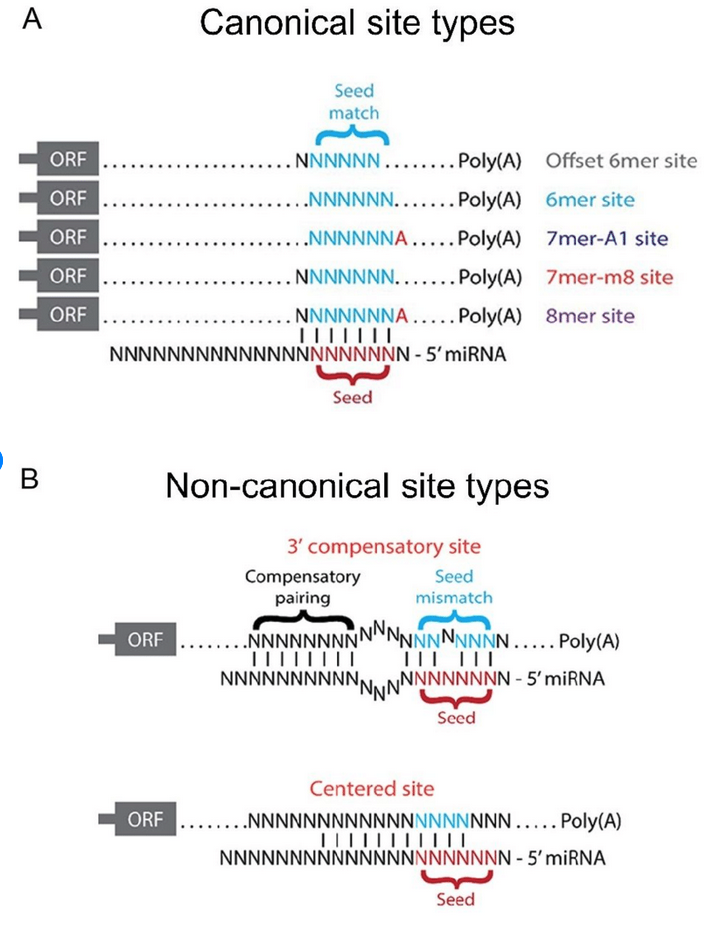
\includegraphics[width=0.5\textwidth]{Figures/canonical_noncanonical}
	\caption{Example of canonical and non-canonical binding sites.}
	\label{fig:canonical_binding}
\end{figure}
